\documentclass{article}
\usepackage[utf8]{inputenc}

\title{Survey on Discrete Wavelet Transforms Using GPU}
\author{Samuel Li}
\date{April 2015}

%\usepackage{natbib}
\usepackage{graphicx}
\usepackage{caption}
\usepackage{subcaption}
\usepackage{color}
\usepackage{setspace}
\newcommand{\fix}[1]{\textcolor{red}{#1}} %Put words in Red

\begin{document}
\onehalfspacing

\maketitle

\begin{abstract}
Discrete Wavelet Transform (DWT) is widely used in data reduction applications.
%
However, such transforms are relatively computationally intensive.
%
To accelerate the calculation of DWT, researchers have applied various parallel
computing techniques, based on the distributed memory architecture~\cite{
chadha2002scalable, nielsen1997scalable}
and the shared memory architecture~\cite{
kutil1999hardware,lucka2000parallel}.
%
In the recent years, the many-core architecture, such as GPU acceleration 
cards, have emerged in the parallel computing field.
%
In this survey paper, we cover many topics regarding calculation of DWT on GPUs.
%
More specifically, we start the survey from technical discussion and evaluation
of implementing the DWT on GPUs~\cite{tenllado2008parallel, van2011accelerating,
garcia2005gpu}.
%
Then we present a few successful use cases of GPU in parallel DWT~\cite{
strengert2004hierarchical, strengert2006pyramid, wong2007discrete,
treib2012turbulence}.
%
Finally, to prepare for the exascale computing, we survey the use of 
heterogeneous architecture with GPUs and multi-core CPUs together,
as well as the GPU clusters~\cite{franco2009parallel, franco2010parallel,
strengert2005large, franco20122d, rossinelli2011multicore}.
%
\end{abstract}

\section{Introduction}

\section{Background of Wavelet Transforms}
Discrete Wavelet Transform (DWT) on a signal $x[n] \: (0 \leq n < N)$ is essentially
passing the signal through a filter function, $f$, 
in a convolution operator.
%
This filter function is also called the \textit{kernel} of this DWT.
%
The results of this DWT are \textit{coefficients} of the signal.
%
The coefficients can be further categorized as two separate groups: 
one representing an approximation of the original signal,
namely \textit{scale coefficients};
and another one contains the detailed information to reconstruct
the original signal from the approximation, namely 
\textit{detail coefficients}.
%
Normally each of these two groups of coefficients has a size $\frac{N}{2}$.


DWTs can also be applied on the coefficients from previous DWTs.
%
When applying another round of DWT, transforms are applied on the two
groups of coefficients separately.
%
As a result, the original singal $x[n]$ is represented as 4 groups of 
coefficients; each has a size $\frac{N}{4}$.
%
This iteration finishes when each of the coefficient groups are small enough,
or the number of iterations reaches the maxinum value set by the user. 
%
%Since a singal is decomposed into multiple groups of coefficients,
%this process is also named a \textit{decomposition}.
%
%Similarly, the reverse calculation, which reconstructs the original signal 
%from the coefficients, is named \textit{reconstruction}.
%
Figure~\ref{fig:example1} illustrates an example of applying DWTs for 
three rounds on an 8-element signal.



\begin{figure}[p]
    \centering
    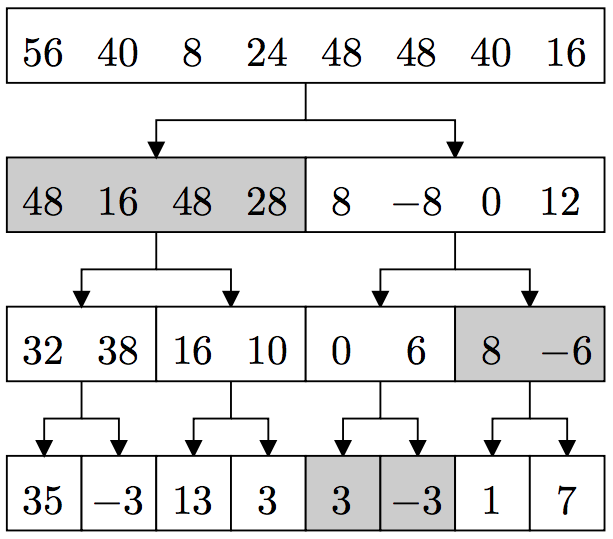
\includegraphics[width=0.8\textwidth]{fig/example1.png}
    \caption{An example of DWT on a signal with 8 elements.}
    \label{fig:example1}
\end{figure}



From the perspective of computational models in parallel computing, 
stencil



\label{sec:bg}

\section{Single Instruction Multiple Data}
The Single Instruction Multiple Data (SIMD) architecture was popular in the
1990s.
%
With SIMD architecture, all processing elements (PE) execute identical instructions
cycle by cycle, but they access different local data from their private 
local memory.
%
All PEs are also connected in a net structure, allowing
communication between them.
%
Figure~\ref{fig:simd1} illustrates an example SIMD architecture.

\begin{figure}
    \centering
    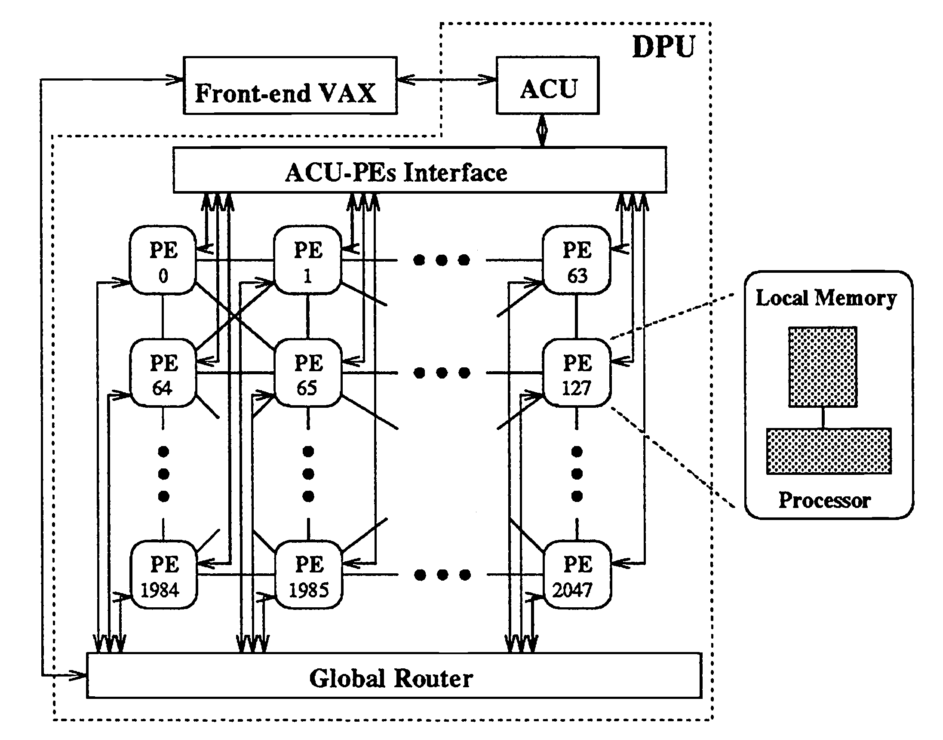
\includegraphics[width=0.8\textwidth]{fig/simd.png}
    \caption{An example of the SIMD architecture: the MasPar system.}
    \label{fig:simd1}
\end{figure}


Lee et. al. implemented DWT on a SIMD machine, the MasPar
system~\cite{lee1994parallel}.
%
MasPar has 2048 PEs organized in a 64x32
mesh topology, as shown in Figure~\ref{fig:simd1}.
%
This implementation takes use of the row structures of available PEs,
by mapping an one-dimensional intput signal onto a row of PEs to process.
%
More specifically, a row of PEs take input values and perform calculations 
togethers, and pass the output coefficients to the next row of PEs.
%
The next row of PEs then perform the next iteration of DWT on the input
coefficients.
%
At the same time, the first row of PEs take in new input to calculate on.
%
This process is illustrated in Figure~\ref{fig:simd2}.


\begin{figure}
    \centering
    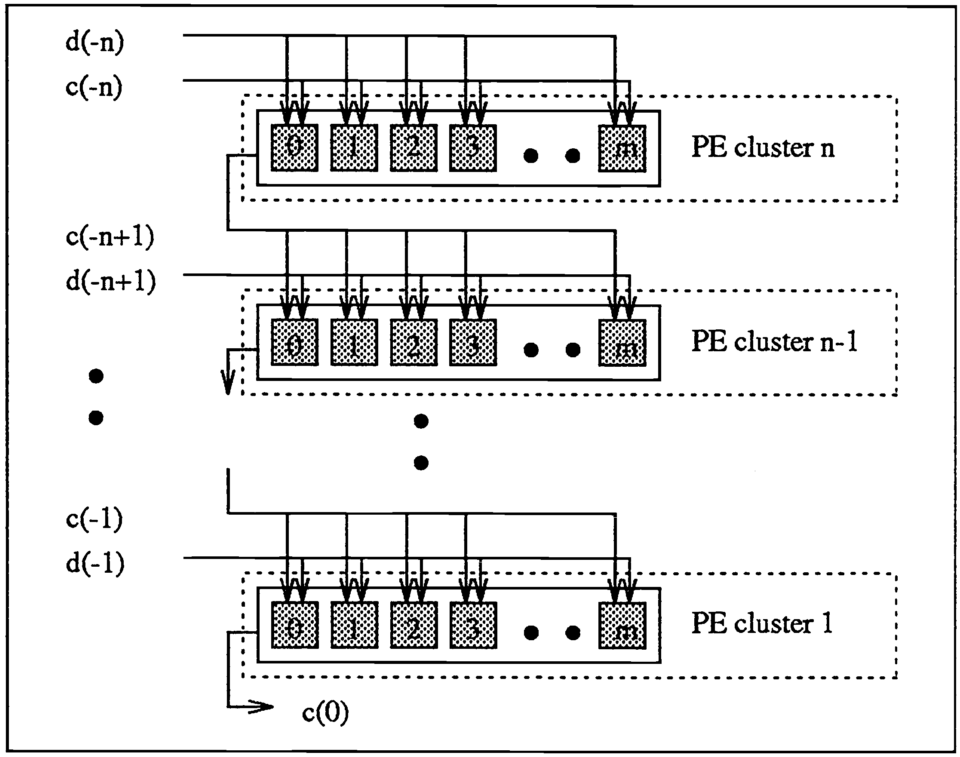
\includegraphics[width=0.8\textwidth]{fig/simd2.png}
    \caption{The pipeline of rows of PEs executing same instructions.
             The output of previous row serves as input for the next row
             of PEs to perform the next iteration of DWT.}
    \label{fig:simd2}
\end{figure}


From the perspective of parallel execution, this implementation uses
a pipeline pattern to achieve great parallelism.
%
As we discussed in class, the amount of parallelism achieved depends on
the number of iterations of DWT we could perform on the input signal.
%
This implementation might not be able to make use of all PEs if run on 
a very large system with many rows of PEs.


The experiment shows that the parallel implementation has a better 
performance than that of a serial implementation on the SPARC 1 workstation,
whose processor is at least 100 times faster than that of the MasPar.
%
Scalability wise, this pipeline implementation is able to keep good speedups
when the problem size grows.
%
This is because larger problems naturally enables more iterations of DWT
to apply on.
%
As a result, the execution pipeline has more steps, and can run more efficiently.

\label{sec:simd}

\section{Shared Memory Architecture}
When performing DWT, the calculation of each coefficients depends only 
on a few input elements from its neighbors (see stencil pattern 
discussion in Section~\ref{sec:bg}).
%
This property makes the calculation of DWT fit in the 
Shared Memory Architecture (SMA) very well, 
by assigning each PE a small chunk of the input signal array
to operate on.
%
Research works from Kutil et. al. and Lucka et. al. both employ
this parallel scheme~\cite{kutil1999hardware, lucka2000parallel}.

Experiments by Kutil et. al. on the SGI POWERChallengeGR machine showed 
a linear speedup up to 10 PEs, while the parallel efficiency drops 
dramatically with more PEs.
%
The researchers than decided that the efficiency was hurt by 
cache misses when more PEs were involved in.
%
These observations and analyses are confirmed by Lucka et. al.
%
Their experiments and analyses showed similar speedup patterns
and performance impact by cache misses.

\label{sec:sma}

\section{Distributed Memory Systems}
Distributed memory systems 

\label{sec:dma}

\section{CUDA architecture}
Traditionally, GPUs are used for fast processing on 
graphics-related calculations.
%
A GPU usually consists of hundreds or thousands of processing elements,
though each is simply focusing on floating point operations. 
%
As a result, a GPU has very high FLOPS to carry out graphics-related
calculations, but lack the ability to 
perform sophisticated operations like a CPU.


More recently, the GPU venders have developed APIs that allow users
to program general-purposed programs on the GPUs. 
%
As a result, the GPUs have become an important architecture in 
parallel computing community.
%
The newest supercomputer ranking, top500, reports that three out of 
top ten supercomputer systems are equipted with GPUs.


Despite the same vision of using GPUs to accelerate the computation,
different venders of GPUs provide different APIs. 
%
The most successful one, Compute Unified Device Architrcture (CUDA), 
is currently from NVIDIA.
%
Our focus will be specifically on the CUDA architecture in the rest 
of this section.


\subsection{Hardware Organization and Programming Model}
\label{sec:cuda-model}
%
With hundreds to thousands of cores and the associated memory, 
a CUDA GPU is organized in its unique way. 
%
Franco et. al. provides a good overview of such 
architecture~\cite{franco2009parallel}.


CUDA cores are organized in two hierarchies in a CUDA GPU:
first a certain number of CUDA cores are grouped together as a multiprocessor,
and second a set of multiprocessor are put together on a CUDA GPU.
%
Here each multiprocessor has a SIMD architecture.


The memory organization on a CUDA GPU is also in hierarchy.
%
In the most fine-grained level, there are registers attached to each CUDA core.
%
The next level memory is \textit{shared memory}, which is shared by all cores
in a multiprocessor.
%
\textit{Device memory} is on the GPU card, and is shared by all the CUDA cores.
%
In addition to shared memories and device memories, there are also dedicated 
memories for particular uses, namely constant cache and texture cache.
%
We are not going to cover these dedicated memories in this survey.
%
At last, the hardware model of a CUDA GPU is shown in Figure~\ref{fig:cuda-hw}.
%

%\begin{figure}
%    \centering
%    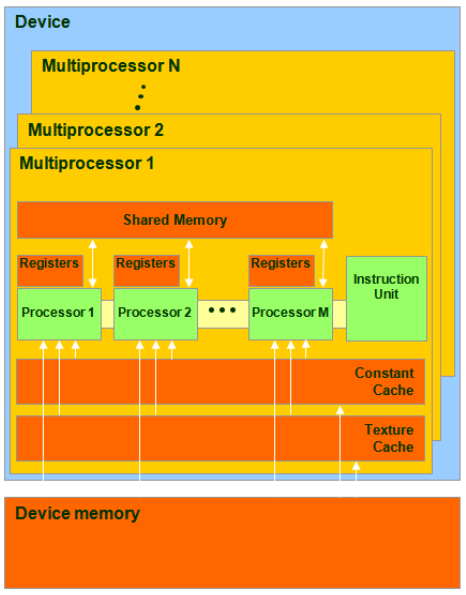
\includegraphics[width=0.8\textwidth]{fig/cuda-hw.png}
%    \caption{Hardware model of a CUDA GPU.}
%    \label{fig:cuda-hw}
%\end{figure}


In the CUDA programming model, a multi-threaded task is partioned into 
many \textit{blocks}.
%
Threads in the same group are executing the same instructions.
%
From the perspective of the program, there could be as many blocks
as necessary.
%
Eventually, each thread is identified using its \textit{threadID} in 
the block, and the \textit{blockID} of that particular block.
%
When executing, each block of threads is mapped to run on one CUDA 
multiprocessor. 
%
This mapping is managed by CUDA to be scalable, meaning that each CUDA 
multiprocessor is always executing a thread block, until the task
is finished~\cite{cudaprogramming}.
%
This CUDA programming model is illustrated in Figure~\ref{fig:cuda-pro}.



\begin{figure}
    \centering
    \begin{subfigure}[b]{0.46\textwidth}
                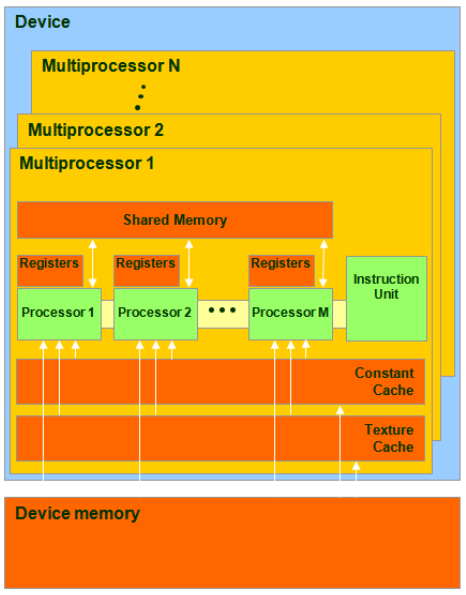
\includegraphics[width=\textwidth]{fig/cuda-hw.png}
                \caption{Hardware model of a CUDA GPU. 
                CUDA cores, multiprocessor, and the GPU card
                make a hierarchy together.}
                \label{fig:cuda-hw}
        \end{subfigure}
\quad
    \begin{subfigure}[b]{0.42\textwidth}
        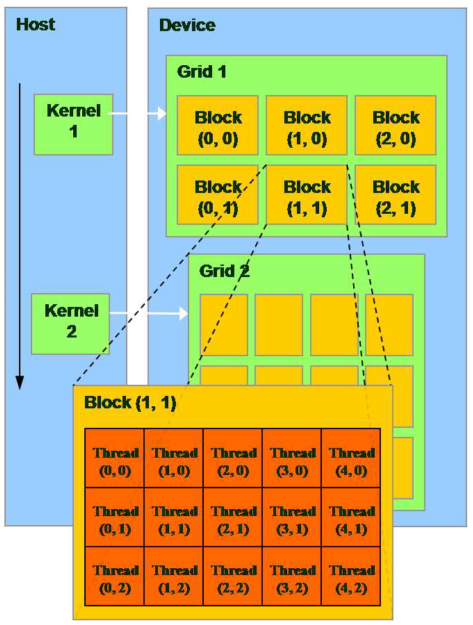
\includegraphics[width=\textwidth]{fig/cuda-pro.png}
        \caption{Programming model on a CUDA GPU.
                 Threadsblocks, and grids make a programming 
                 hierarchy.}
        \label{fig:cuda-pro}
    \end{subfigure}
%
    \caption{CUDA hardware and programming model.}
\end{figure}



\subsection{Naive Parallelism using CUDA}
\label{sec:cuda-naive}
%
Franco et. al.~\cite{franco2009parallel} parallelized two-dimensional 
DWT following the similar approach
illustrated in the top diagram of Figure~\ref{fig:c}.
%
More specifically, the researchers identified two sections of DWT
that could be paralllized: the one-dimensional DWT on rows, and the
matrix transpose.
%
When implementing such algorithms using CUDA, the program specifies
sections to run on the GPU as \textit{kernels}, and pass the data 
as well as operations onto the GPU to execute.
%
The calculation results from GPU executions are then copied back
to continue this algorithm for further operations.

Experiment results show that the CUDA implementation of 
two-dimensional DWT on an NVIDIA Tesla C870 GPU achieves 
10x to 21.7x speedups, compared to the optimized implementation 
on an Intel Core 2 Quad CPU.
%
A breakdown of the total calculation time further shows that 
the two data transfer steps, which move data from system main memory
to the GPU to perform DWT and matrix transpose, take around half
of the total elapsed time.
%
This result indicates that reducing data movement between the GPU and 
system main memory is a direction to further increase performance.  


\subsection{To Make Better Use of Blocks in CUDA}
%
Lann et. al. investigated better use of the blocks in CUDA,
and proposed a different way to partition the input data to fit in
this model~\cite{van2011accelerating}.
%
This section is going to briefly introduce two different approaches 
the researchers use to perform DWT on rows and columns.



When an algorithm designer makes decisions to move multi-threaded tasks
to the GPU, one always needs to partition the problem carefully,
with the consideration of memory operations.
%
Specifically, the \textit{coalesced} reads and writes,
meaning that reads and writes of a continuious chunk of memory,
are always preferable.
%
In a two-dimensional data set that is stored in a row-oriented fashion,
accessing data row by row naturally implies coalesced reads and writes,
but column by column results in discrete random data access.
%
As a result, Lann et. al. designed different data partitioning schemes 
for DWT on rows and on columns.


In the first case of DWT on rows, the researchers partitioned the 
two-dimensional data into many 1D arrays, each representing one row
from the original data set.
%
Each array is then mapped onto one block in the CUDA programming model.
%
Figure~\ref{fig:cuda-row} illustrates this approach: 
each thread block performs DWT on one row of input data.
%
The black squares indicate that one thread moves along the row
as the block calculates DWT in the one-dimension fashion.


In the second case of DWT on columns, a simple partition of every column
would not work well, because of the discrete memory access.
%
The researchers then decided to partition the data in ``slabs,"
rather than single columns, to map to the programming blocks.
%
Figure~\ref{fig:cuda-column} compares this partitioning with 
the partitioning for DWT on rows.


Experiments showed that DWT on columns using this ``slab"-like 
partitioning performs only $10\%$ to $20\%$ slower than DWT on rows.
%
The researchers also compared this approach to the one in 
Section~\ref{sec:cuda-naive}, which involves a matrix transpose
and then performs DWT on columns just in consecutive memories.
%
The results are still in favor of their approach --- the total
execution time is 2x to 2.5x faster than the approach that involves
matrix transpose.

\begin{figure}
    \centering
    \begin{subfigure}[b]{0.85\textwidth}
                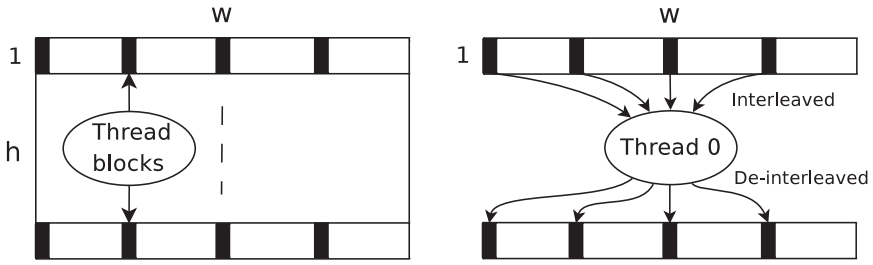
\includegraphics[width=\textwidth]{fig/row.png}
                \caption{
                Data partition of the two-dimensional data set onto 
                blocks in a GPU programming model to perform DWTs on rows.
                %
                Each row is mapped to a block in this figure, and the black
                square shows a thread process data along this row. 
                }
                \label{fig:cuda-row}
        \end{subfigure}
\quad
    \begin{subfigure}[b]{0.85\textwidth}
        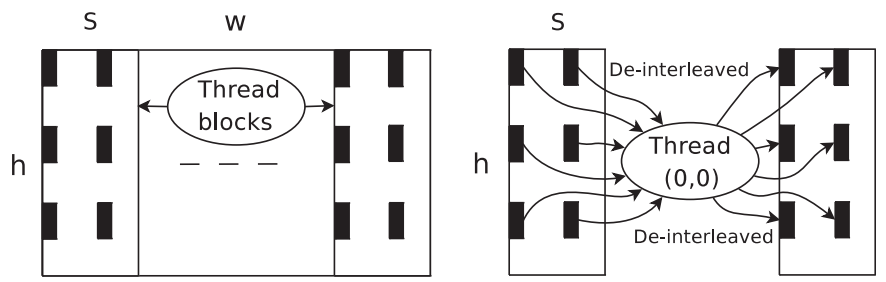
\includegraphics[width=\textwidth]{fig/column.png}
        \caption{
                Data partition of the two-dimensional data onto 
                blocks in a GPU programming model to perform DWTs on columns.
                %
                Each block contains $S$ columns together in this figure.
                }
        \label{fig:cuda-column}
    \end{subfigure}
%
    \caption{Different data partitioning schemes for DWT on rows and columns.}
\end{figure}






\label{sec:cuda}

\bibliographystyle{plainyr} 
%\bibliographystyle{plain}
\bibliography{main}
\end{document}

